% -*- latex -*-
%%%%%%%%%%%%%%%%%%%%%%%%%%%%%%%%%%%%%%%%%%%%%%%%%%%%%%%%%%%%%%%%
%%%%%%%%%%%%%%%%%%%%%%%%%%%%%%%%%%%%%%%%%%%%%%%%%%%%%%%%%%%%%%%%
%%%%
%%%% This text file is part of the source of 
%%%% `Parallel Programming in MPI and OpenMP'
%%%% by Victor Eijkhout, copyright 2012-9
%%%%
%%%% mpi-io.tex : MPI/O
%%%%
%%%%%%%%%%%%%%%%%%%%%%%%%%%%%%%%%%%%%%%%%%%%%%%%%%%%%%%%%%%%%%%%
%%%%%%%%%%%%%%%%%%%%%%%%%%%%%%%%%%%%%%%%%%%%%%%%%%%%%%%%%%%%%%%%

\index{MPI/O|(}

File input and output in parallel is a little more complicated than
sequentially.
\begin{itemize}
\item There is nothing against every process opening an existing file
  for reading, and using an individual file pointer to get its unique
  data.
\item \ldots~but having every process open the same file for output is
  probably not a good idea.
\item Based on the process rank it is easy enough to have
  every process create a unique file, but that can put a lot of strain
  on the file system, and it means you may have to post-process 
  to get all the data in one file.
\end{itemize}

Wouldn't it be nice if there was a way to open one file in parallel,
and have every process read from and write to its own location? That's
where \emph{MPI/O} comes in.

There are dedicated libraries for file I/O, such as \indexterm{hdf5},
\indexterm{netcdf}, or \indexterm{silo}. However, these often add
header inforation to a file that may not be understandable to
post-processing applications. With MPI I/O you are in complete control
of what goes to the file. (A~useful tool for viewing your file is the
unix utility~\indextermtt{od}.)

\Level 0 {File handling}

MPI has its own file handle:
\mpiRoutineRef{MPI_File}

File open:
%
\mpiRoutineRef{MPI_File_open}
%
This routine is collective, even if only certain processes will access
the file with a read or write call.
Similarly, \indexmpishow{MPI_File_close} is collective.

\begin{pythonnote}
  Note the slightly unusual syntax for opening a file: even though the file is
  opened on a communicator, it is a class method for the \n{MPI.File}
  class, rather than for the communicator object. The latter is passed
  in as an argument.
\end{pythonnote}

File access modes:
\begin{itemize}
\item  \indexmpishow{MPI_MODE_RDONLY}: read only,
\item  \indexmpishow{MPI_MODE_RDWR}: reading and writing,
\item  \indexmpishow{MPI_MODE_WRONLY}: write only,
\item  \indexmpishow{MPI_MODE_CREATE}: create the file if it does not exist,
\item  \indexmpishow{MPI_MODE_EXCL}: error if creating file that already exists,
\item  \indexmpishow{MPI_MODE_DELETE_ON_CLOSE}: delete file on close,
\item  \indexmpishow{MPI_MODE_UNIQUE_OPEN}: file will not be concurrently opened
  elsewhere,
\item  \indexmpishow{MPI_MODE_SEQUENTIAL}: file will only be accessed sequentially,
\item  \indexmpishow{MPI_MODE_APPEND}: set initial position of all file pointers to end
  of file.
\end{itemize}
These modes can be added or bitwise-or'ed.

You can delete a file with \indexmpishow{MPI_File_delete}.

\Level 0 {File access}

Writing to and reading from a parallel file is rather similar to
sending a receiving:
\begin{itemize}
\item The process uses an elementary data type or a derived datatype
  to describe what elements in an array go to file, or are read from
  file.
\item In the simplest case, your read or write that data to the file using an
  offset, or first having done a seek operation.
\item But you can also set a `file view' to describe explicitly what
  elements in the file will be involved.
\end{itemize}

File accesses:
\begin{itemize}
\item \indexmpishow{MPI_File_seek}
\item \indexmpishow{MPI_File_read}
\item \indexmpishow{MPI_File_read_all}
\item \indexmpishow{MPI_File_read_ordered}
\item \indexmpishow{MPI_File_read_shared}
\item \indexmpishow{MPI_File_read_at}: combine read and seek.
\item \indexmpishow{MPI_File_write}
\item \indexmpishow{MPI_File_write_all}
\item \indexmpishow{MPI_File_write_ordered}
\item \indexmpishow{MPI_File_write_shared}
\item \indexmpishow{MPI_File_write_at}: combine write and seek
\end{itemize}

\begin{figure}[ht]
  \label{fig:write-at}
  \caption{Writing at an offset}
  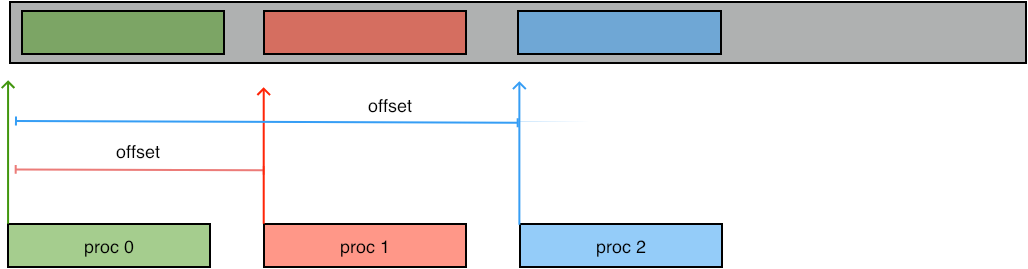
\includegraphics[scale=.4]{write-at-offset}
\end{figure}

\begin{exercise}
  \label{ex:blockwrite}
  Create a buffer of length \n{nwords=3} on each process, and write
  these buffers as a sequence to one file with \indexmpishow{MPI_File_write_at}.
\end{exercise}

These modes are enough for writing simple contiguous blocks. However,
you can also access non-contiguous areas in the file. For this you use
%
\mpiRoutineRef{MPI_File_set_view}
%
This call is collective, even if not all processes access the file.
\begin{itemize}
\item The \n{etype} describes the data type of the file, it needs to
  be the same on all processes.
\item The \n{filetype} describes how this process sees the file, so it
  can differ between processes.
\item The \n{disp} displacement parameters is measured in bytes. It
  can differ between processes. On sequential files such as tapes or
  network streams it does not make sense to set a displacement; for
  those the \indexmpidef{MPI_DISPLACEMENT_CURRENT} value can be
  used.
\end{itemize}

\begin{figure}[ht]
  \label{fig:write-view}
  \caption{Writing at a view}
  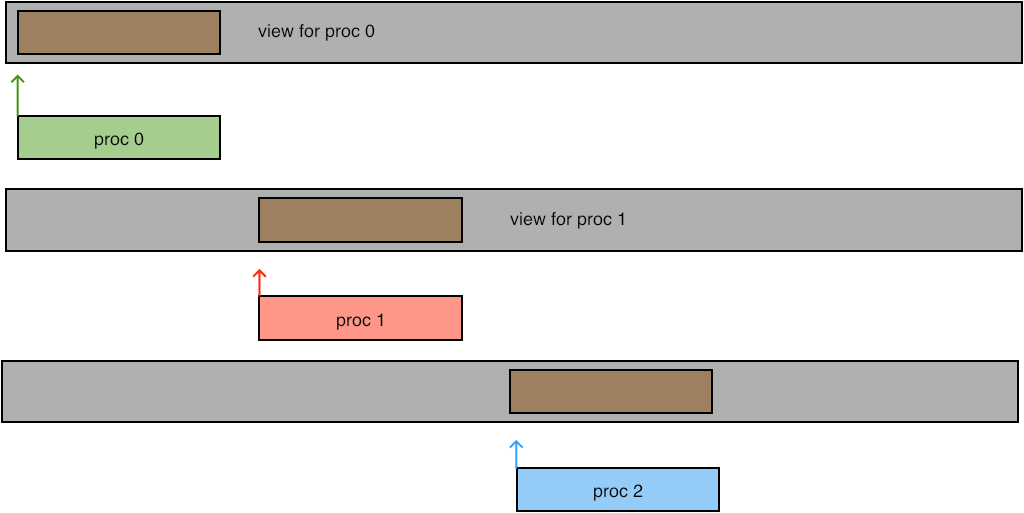
\includegraphics[scale=.4]{write-at-view}
\end{figure}

\mpiRoutineRef{MPI_File_write_at}

\begin{exercise}
  \label{ex:viewwrite}
  Write a file in the same way as in exercise~\ref{ex:blockwrite},
  but now use \indexmpishow{MPI_File_write} and use \indexmpishow{MPI_File_set_view} to set
  a view that determines where the data is written.
\end{exercise}

You can get very creative effects by setting the view to a derived
datatype.

\begin{figure}[ht]
  \label{fig:write-derived}
  \caption{Writing at a derived type}
  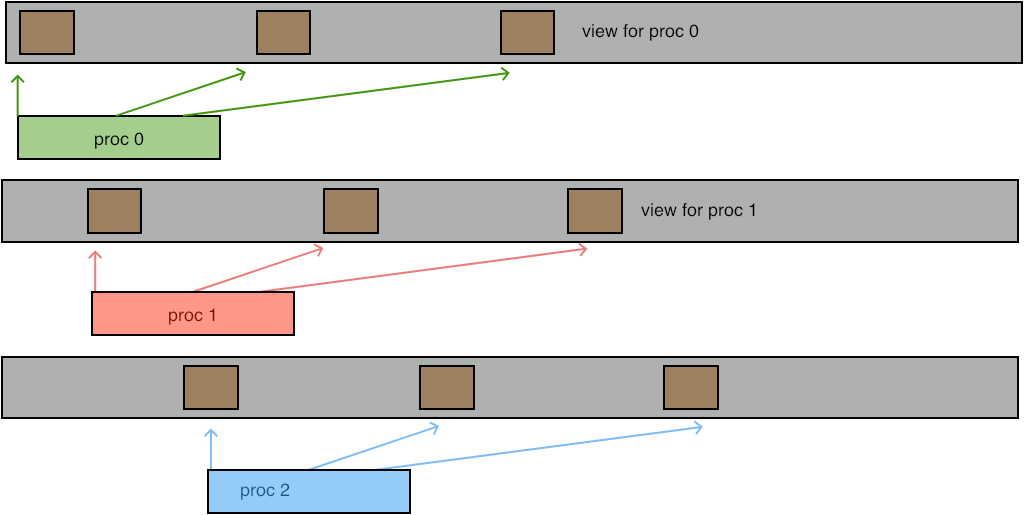
\includegraphics[scale=.4]{write-at-derived}
\end{figure}

\begin{fortrannote}
  In Fortran you have to assure that the displacement parameter is of
  `kind' \indexmpi{MPI_OFFSET_KIND}. In particular, you can not
  specify a literal zero~`0' as the displacement; use
  \indexmpidef{0_MPI_OFFSET_KIND} instead.
\end{fortrannote}

More:
\indexmpishow{MPI_File_set_size}
\indexmpishow{MPI_File_get_size}
\indexmpishow{MPI_File_preallocate}
\indexmpishow{MPI_File_get_view}

\Level 0 {Constants}

\indexmpishow{MPI_SEEK_SET} used to be called \indextermtt{SEEK_SET}
which gave conflicts with the C++ library. This had to be circumvented
with
\begin{verbatim}
make CPPFLAGS="-DMPICH_IGNORE_CXX_SEEK -DMPICH_SKIP_MPICXX"
\end{verbatim}
and such.

\index{MPI/O|)}
